\section{Closest Pair of Points in 2D}

\subsection{Expected Number of Reboots}

Assume that the points are randomly shuffled at the start but not after each reboot--if we go up to the $i$-th element and rebooted, the first $i$ elements we draw after the reboot will be the same. This means that if we had to reboot after observing the $k$-th element, we will never reboot at the $k$-th element again. Also assume that the closest pair is unique.

Consider the probability of rebooting after observing the $i$-th point $p_i$. This is the same as the probability of $p_i$ being part of a closest pair with another point in the first $i$ points which is $2/i$ since we have looked at $i$ points and $p_i$ could be at either end of the closest pair. Since the $p_1$ and $p_2$ do not cause a reboot since they give the starting $r$,
\[
  \mathbf{E}[\text{Number of reboots}] = \sum_{i=3}^n \frac{2}{i} = 2H_n - 3
\]
where $H_n$ is the $n$-th harmonic number.

\subsection{Real-World Performance}

Since the asymptotic running time is already given for both algorithms, we will focus on the theoretical space usage. The divide and conquer version operates mainly on slices of the input array and creates a new, temporary vector only for the band. So, the space usage should just be the size of the input---$O(n)$. The linear version requires us to keep track of a grid so it would require an extra $O(n)$ space. However, the linear version's memory footprint is expected to be more sparse since the grid works like a map so each of the bin could be more largely scattered around memory in contrast to the slices or vectors of bands that are contiguous in memory.

The implementations can be found \href{https://github.com/nngerncham/cs315_private/tree/main/final/cp_code02}{here}. It should become public after the due date for the exam. The idea for the implementation of linear-time closest pair is based on \href{https://www.cs.cmu.edu/~15451-s15/LectureNotes/lecture16/closest-pair.pdf}{this lecture note} on closest pairs from CMU. Both implementations also use the square distance of integer points in 2D defined by $dist(p_1 := (x_1, y_1), p_2 := (x_2, y_2)) = (x_1 - x_2)^2 + (y_1 - y_2)^2$. 1,000, 10,000, 100,000, and 1,000,000 integer points were generated randomly and thrown into each algorithm for benchmarking. The results are as follows.

\begin{figure}[h]
	\centering
	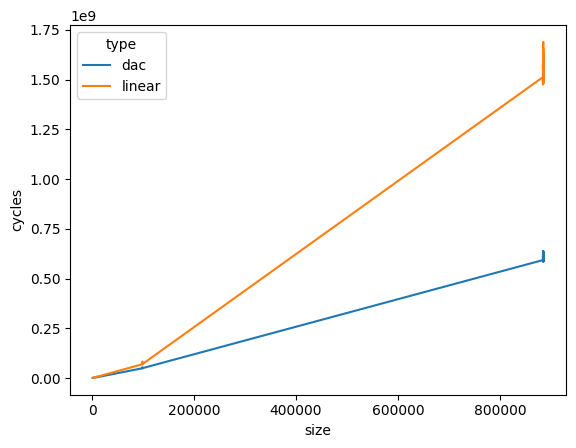
\includegraphics[width=0.7\textwidth]{graphics/graph.png}
	\caption{Benchmarking results of both algorithms}
\end{figure}

\subsection{Discussion}

From the plot, we can see that the divide and conquer (dac) version outperforms the randomized linear version by a lot which is rather surprising given that the asymptotic running time indicates that it should be the other way around.

As discussed above, the reason behind why the real world running time is so much worse could be due to the memory usage. The grid where bins are represented as a HashMap could become very large and sparse, causing each bin to possibly be quite far from each other. This leads to higher cache miss rates leading to worse performance. The rebuilding of the grid after each reboot could also be so much more expensive in the real world compared to asymptotically since it could involve a lot of memory allocation for all the new \textit{bins} that need to be rehashed. Obviously, the speed of hashing a point (tuple of two integers) could also have affected the running time as well.

Another big reason for this could just be due to the rather naive implementation of the grid API. There could be ways of implementing a more efficient grid API but there was not enough time to explore that. As such, the linear version could be held back due to the inefficiency of the grid API so running time could be improved if the grid API was more efficient.
